\documentclass[  12pt,
titlepage,
parskip,
draft=false,
headsepline=true,
footsepline=true,
captions=tableheading]{scrartcl}
\usepackage[english]{babel}
\usepackage{csquotes}
\usepackage[utf8]{inputenc}
\usepackage[a4paper , lmargin = {2.5cm} , rmargin = {2.5cm} , tmargin = {2.5cm} , bmargin = {2.5cm}]{geometry}
\usepackage[hyphens]{url}
\usepackage[linktocpage=true]{hyperref}
\usepackage{tabularx}
\usepackage{amsmath}
\usepackage[backend=biber,style=authoryear,sortcites=false,citestyle=authoryear]{biblatex}
\bibliography{Literatur.bib}%Dateiname für Quellen einfügen
\usepackage{ragged2e} %für bessere URL formatierung bei printbibliography

%Bilder einbinden und es ermöglich auf der gleichen seite ein
%Fußnotenzitat einzufügen
\usepackage{graphicx}
\usepackage{float}
\usepackage{afterpage}
\interfootnotelinepenalty=99999 %Seitenumbruch einer Fußzeile verhindern

\usepackage{moreverb} %tabulator formatierung in verbatim umgebung

%nur einzelne Kapitel einbinden:
%\includeonly{2_Umfeld.tex}
%\includeonly{3_Grundlagen_IT-IST-Analyse.tex}


\renewcommand{\labelenumi}{\arabic{enumi}.}
\renewcommand{\labelenumii}{\arabic{enumi}.\arabic {enumii}}
\renewcommand{\labelenumiii}{\arabic{enumi}.\arabic{enumii}.\arabic{enumiii}}

\newcommand{\firstpages}{
	% !TEX root = Thesis.tex

\thispagestyle{empty}
\vspace{1cm}

\begin{center}
\Large{Hochschule für Telekommunikation Leipzig (FH)}
\vspace{1.5cm}
\end{center}

\begin{center}
\large{\textbf{Abschlussarbeit zur Erlangung des akademischen Grades}}
\end{center}

\begin{center}
\vspace{-2mm}
 \Large\textbf{Bachelor of Science}
\end{center}

\begin{center}
\vspace{5mm}
\textbf{im Studiengang Wirtschaftsinformatik}
\end{center}

\vspace{3cm}
\begin{tabular}{p{0.2\textwidth}p{0.7\textwidth}}
\textbf{Thema:} & 
	Exploring the offshoring approach of German Companies compared to  to the U. S. American approach

\\
&
	
\\ &
\\ &
\\

\vspace{4,5cm}\\

\textbf{Vorgelegt von:} & Veronika Lawrence \\ 
&\\
&\\
&\\
&\\
\textbf{geboren am:} & 31. Oktober 1991 \\
\textbf{in:} & Starnberg \\
\textbf{Matrikelnummer: } & {}134130\\
&\\

\textbf{eingereicht am:} & 15. Oktober 2016 \\
&\\
&\\
&\\
\textbf{Themensteller:} & T-Systems International\\
& Systems Integration\\
& SAP Technology \& Analysis\\
& \\

\textbf{Erstprüfer:} & Prof. Dr. Christian Czarnecki \\
&\\
&\\

\textbf{Zweitprüfer:} & [Titel einfügen]Thomas Vogt \\
\end{tabular}
 
	
	\newpage
	\tableofcontents{}
	\addtocontents{toc}{~\hfill\textbf{Page}\par}
	
	\newpage
	\listoffigures
	
	\newpage
	\listoftables
	\newpage
}
\begin{document}
\pagenumbering{gobble}
\firstpages

\pagenumbering{arabic}
\section{Introduction}

\newpage
\section{Offshoring in literature}
Offshoring has been widely studied in the past decades. There are two major branches of research: the first describes reality through statistics or case studies (e.g. \cite{Rottman.2008}, \cite{Pedersen.2013} )

\subsection{Definition and Terms}
In existing literature, there is no single definition of the term offshoring nor a precise delimitation to the term outsourcing. Both apply to organizational decisions in companies. 

According to \cite[pp. 1f]{Specht.2007}, outsourcing is buying services from other companies. Offshoring is defined as a special form of outsourcing, in which the service is bought from a foreign company. \cite[p. 2]{Alebrand.2013} defines outsourcing and offshoring as mutually exclusive: outsourcing is the provision of services by external companies, offshoring is the internal execution of tasks in a foreign country.

These contrasting definitions may serve as an example for the lack of distinct terms in this field of research. Nevertheless all the definitions agree that outsourcing pertains to external service provision and offshoring refers to service provision in a foreign country. This synopsis as well as the planned Bachelor's thesis will use the following definition of the term offshoring by \cite[p. 321]{Andersson.2016}:

%\begin{quote}
%	``Offshoring [is the] disintegration of the firms’ production processes across national borders[...]''
%\end{quote} 

Therefore, the terms offshoring and outsourcing do not have a direct relation; both terms are independent and describe different possibilities of entrepreneurial organization. In figure \ref{fig:DefTerms}, the delimitation between outsourcing and offshoring is clearly shown.

\begin{figure}[htb]
	\centering
	\includegraphics[width=0.7\textwidth]{Pictures/Terms_definition}
	\caption{Definition of terms, based on \cite[pp. 552f]{Antras.2004}}
	\label{fig:DefTerms}
\end{figure}



\subsection{History of Offshoring}
%Enabling Technologies
%

\subsection{Offshoring in the USA}

\subsubsection{Prevalence}

\subsubsection{Offshoring functions}

\subsection{Offshoring in Germany}

\subsubsection{Prevalence}

\subsubsection{Offshored functions}

\subsection{Significant differences between Germany and the USA}

\subsubsection{Difference 1}

\subsubsection{Difference 2}

\newpage
\section{Case Studies}

\subsection{Interview Technique}
%TODO evtl kürzer fassen
In order to complement theoretical findings from literature research, expert interviews have been conducted. A structure for the interviews has been defined (see appendix). In this way, statements from different experts can be compared and evaluated, which allows for a comprehensive review. Even though interviewees may share their native language (German) with the interviewer, interviews have always been conducted in English. Thus, any inaccuracies that may occur during translating the statements were prevented and comparability of interviews has been improved.

The interviews were held remotely, either via an Internet VoIP-Service such as Skype, or via using WebEx, the standard communication platform used at T-Systems when interviewing employees of this company. Considering the often tight schedules of experts in their fields, the duration of interviews was limited to 45 minutes.

To further document the interviews and the steps leading up to them as well as the steps of refinement that follow, a process (see figure \ref{fig:Intprocess}) has been defined adhered to. 

\begin{figure}[htb]
	\centering
	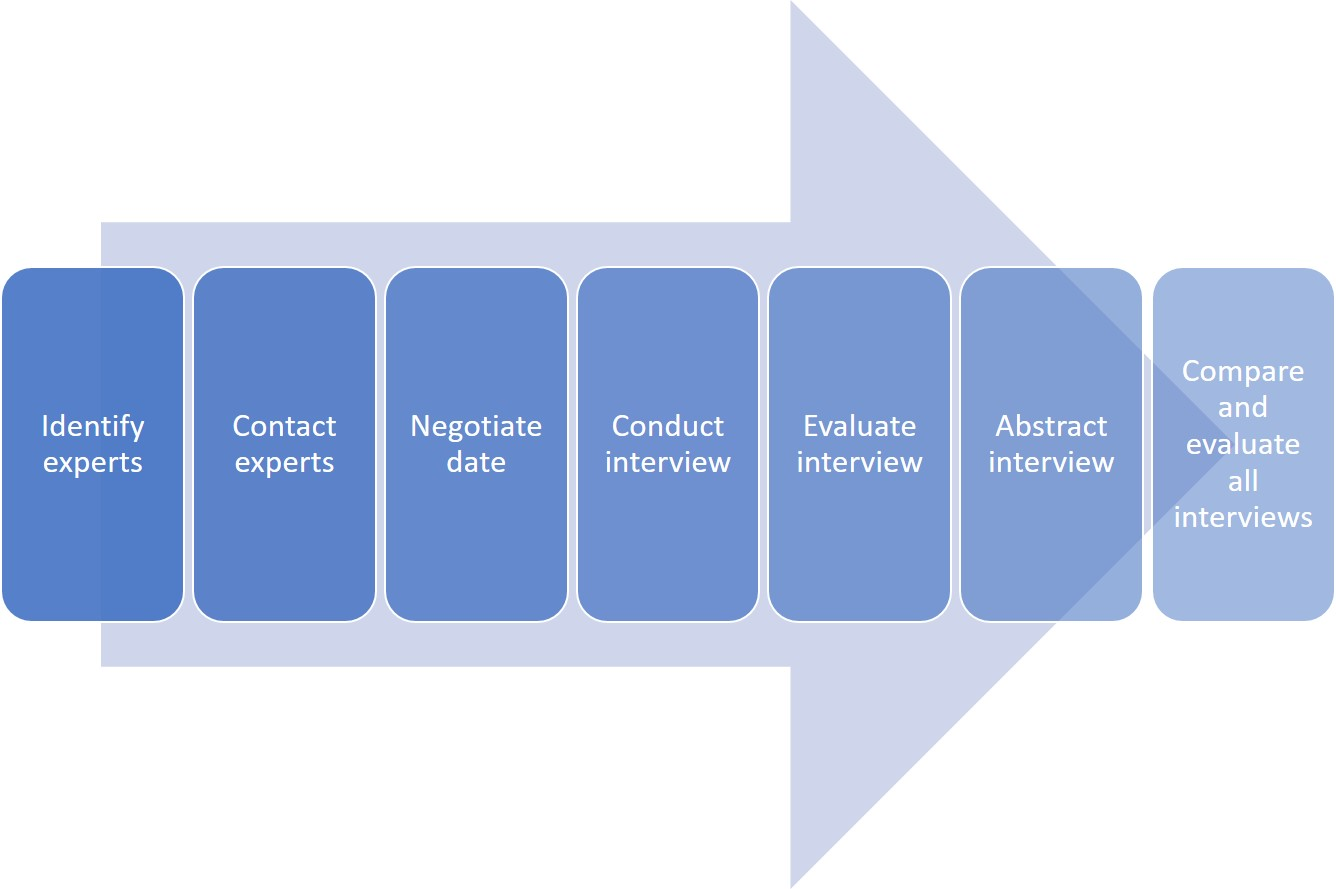
\includegraphics[width=0.7\textwidth]{Pictures/Interview_process}
	\caption{Interview process}
	\label{fig:Intprocess}
\end{figure}

\paragraph{Identify experts} The experts are identified by conducting a network-based search. Initial contacts are asked to identify persons they consider an expert on the topic, who are in turn asked to provide further contacts.
\paragraph{Contact experts} Initial contact to the expert is established via an email sent by the expert's contact. Included is a standard email explaining the topic, duration and process of the interview and providing the researchers' contact details.
\paragraph{Negotiate date} Once the expert has agreed to participate in the interview, the researcher contacts them directly in order to set up date, time and method of communication for the interview. Note that all interviews are conducted using at least voice-based communication. Video can be added to further facilitate the communication between the expert and the researcher.
\paragraph{Conduct interview} The interviews are conducted in five phases with defined leading questions. This means, the leading questions will be asked, but the researcher will also ask further questions as appropriate to the course of the interview. These phases are:
%\begin{itemize}
%	\item Introduction
%	\item Offshoring Experiences in the USA
%	\item Offshoring Experiences in Germany
%	\item Comparison of Experiences in Germany and the USA
%	\item Finalization
%\end{itemize}
During the interview, audio and, if applicable, video will be recorded.

\paragraph{Transcribe interview} The interviews are transcribed by the researcher. These transcriptions are added to the appendix of the thesis and provide the primary source for the origin of statements.

\paragraph{Evaluate interview} The transcriptions are evaluated and any important passages are highlighted. Transcriptions are added to the appendix.

\paragraph{Abstract interview} For each interview, an abstract is developed. The abstracts are included in the thesis.

\paragraph{Compare and evaluate all interviews} Finally, an overview and comparison of all interviews is generated to derive common statements and areas of disagreement.


\subsection{Case Study Title 1}

\subsubsection{Background}
\subsubsection{Results of Interview}
\subsubsection{Conclusions}
\subsection{Case study Title 2}
\subsubsection{Background}
\subsubsection{Results of Interview}
\subsubsection{Conclusions}


\subsection{Summary and Evaluation}

\newpage
\section{Conclusions and Limitations}

\clearpage
\addcontentsline{toc}{section}{References}
\label{Ref}
\printbibliography
\end{document}